\chapter{以斯帖记}
\begin{table}[H]
\centering 
\begin{tabular}{p{1.5cm}|p{16cm}}
\hline
\hline
时间 &事件 \\\hline
元年&亞哈隨魯在書珊城的宮登基 \\\hline
\multirow{3}{1.6cm}{第三年}&為他一切首領臣僕在書珊城設擺筵席一百八十日\\ \cline{2-2}
&為所有住書珊城的大小人民在御園的院子裡設擺筵席七日\\ \cline{2-2}
&第七日,王后瓦實提被废\\ \hline
第四？年&詔選美女為后，以斯帖也送入王宮\\ \hline
第五？年&潔淨身體十二個月\\ \hline
第七年&以斯帖被引入宮見王，十月（提別月）以斯帖被立為王后，代替瓦實提\\ \hline
\multirow{6}{1.6cm}{第十二年}&正月（尼散月）人在哈曼面前掣籤要滅絕所有的猶大人\\ \cline{2-2}
&正月十三日，哈曼吩咐將猶大人全然剪除，殺戮滅絕奪取他們的財為掠物\\ \cline{2-2}
&三月（西彎月）二十三日,末底改寫諭旨,猶大人在一日之間聚集保護性命，剪除仇敵，奪取他們的財物\\ \cline{2-2}
&十二月（亞達月）十三日,猶大人反倒轄制仇敵。猶大人都聚集保護性命，殺了七萬五千，沒有奪取財物 \\ \cline{2-2}
&十二月（亞達月）十四日書珊的猶大人又聚集在書珊，殺了三百人，卻沒有下手奪取財物\\ \cline{2-2}
&十二月（亞達月）十五日安息，以這日為設筵歡樂的日子\\ \hline
\end{tabular}
\caption{时间顺序}
\end{table}

\begin{figure}[H]
  \centering
    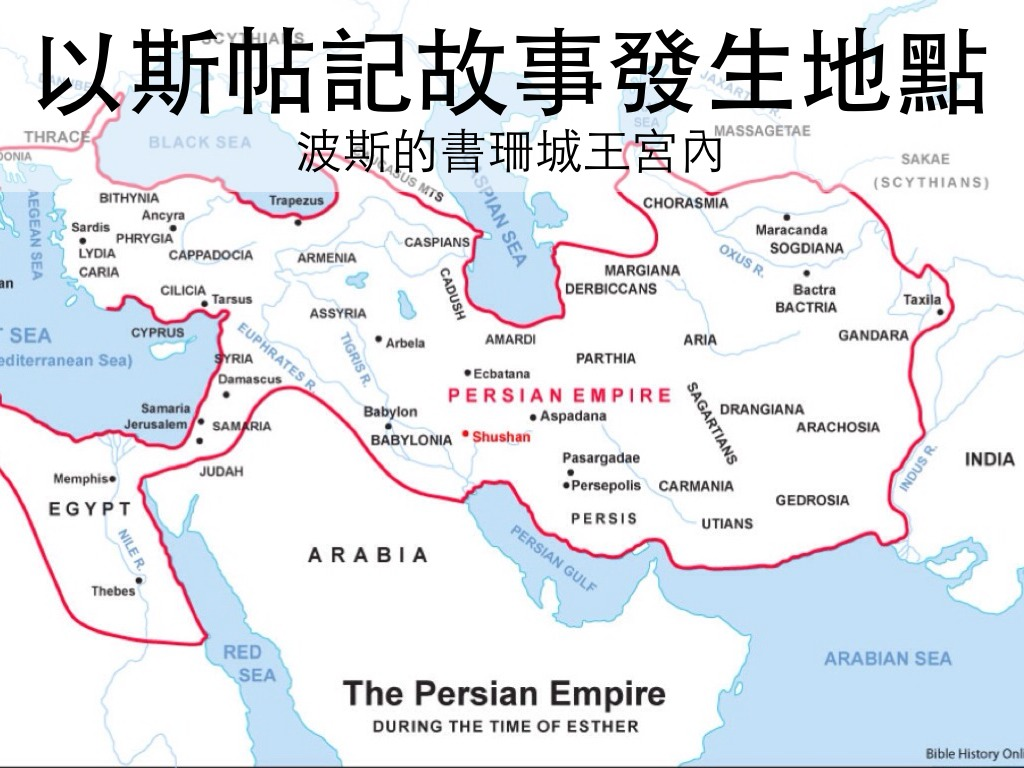
\includegraphics[width=0.9\textwidth]{CBeiLuFigs/shushan0}
      %\caption{以斯帖发生地点}
\end{figure}


\section{王第三年王后瓦實提被废 1}
\subsection{亞哈隨魯三年在書珊城設筵一百八十日 1:1-9}
\begin{table}[H]
  \centering 
    \begin{tabular}{p{20.em}|p{27.em}}    \toprule
一百八十日首領、臣僕&七日書珊城大小人民\\    \midrule
亞哈隨魯做王，從印度直到古實，統管一百二十七省。亞哈隨魯王在書珊城的宮登基，在位第三年，為他一切首領、臣僕設擺筵席，有波斯和瑪代的權貴，就是各省的貴胄與首領在他面前。他把他榮耀之國的豐富和他美好威嚴的尊貴給他們看了許多日，就是一百八十日。
&這日子滿了，又為所有住書珊城的大小人民，在御園的院子裡設擺筵席七日。有白色、綠色、藍色的帳子，用細麻繩、紫色繩從銀環內繫在白玉石柱上。有金銀的床榻，擺在紅、白、黃、黑玉石鋪的石地上。用金器皿賜酒，器皿各有不同，御酒甚多，足顯王的厚意。喝酒有例，不准勉強人，因王吩咐宮裡的一切臣宰，讓人各隨己意。\\     \bottomrule
    \end{tabular} 
\end{table} 


\subsection{王后瓦實提拒遵王命,王甚發怒 1:10-12}
王后瓦實提在亞哈隨魯王的宮內，也為婦女設擺筵席。 10 第七日，亞哈隨魯王飲酒，心中快樂，就吩咐在他面前侍立的七個太監米戶幔、比斯他、哈波拿、比革他、亞拔他、西達、甲迦， 11 請王后瓦實提頭戴王后的冠冕到王面前，使各等臣民看她的美貌，因為她容貌甚美。 12 王后瓦實提卻不肯遵太監所傳的王命而來，所以王甚發怒，心如火燒。

\subsection{王后瓦實提被废 1:13-22}
\begin{table}[H]
\centering 
\begin{tabular}{p{37.em}|p{11.em}}    \toprule
波斯和瑪代的七個大臣&王\\  \midrule
那時，在王左右常見王面，國中坐高位的，有波斯和瑪代的七個大臣，就是甲示拿、示達、押瑪他、他施斯、米力、瑪西拿、米母干，都是達時務的明哲人。按王的常規，辦事必先詢問知例明法的人。
&王問他們說：「王后瓦實提不遵太監所傳的王命，照例應當怎樣辦理呢？」\\\midrule    
米母干在王和眾首領面前回答說：「王后瓦實提這事不但得罪王，並且有害於王各省的臣民。因為王后這事必傳到眾婦人的耳中，說：『亞哈隨魯王吩咐王后瓦實提到王面前，她卻不來。』她們就藐視自己的丈夫。今日波斯和瑪代的眾夫人聽見王后這事，必向王的大臣照樣行，從此必大開藐視和憤怒之端。王若以為美，就降旨寫在波斯和瑪代人的例中，永不更改，不准瓦實提再到王面前，將她王后的位分賜給比她還好的人。 所降的旨意傳遍通國（國度本來廣大），所有的婦人，無論丈夫貴賤，都必尊敬他。」&王和眾首領都以米母干的話為美，王就照這話去行，發詔書，用各省的文字、各族的方言通知各省，使為丈夫的在家中做主，各說本地的方言。\\\bottomrule
\end{tabular} 
\end{table} 


\section{第七年十月以斯帖被立為王后 2}
\subsection{亞哈隨魯下令寻找新王后 2:1-4}
這事以後，亞哈隨魯王的憤怒止息，就想念瓦實提和她所行的，並怎樣降旨辦她。 2 於是王的侍臣對王說：「不如為王尋找美貌的處女。 3 王可以派官在國中的各省招聚美貌的處女到書珊城（宮）的女院，交給掌管女子的太監希該，給她們當用的香品。 4 王所喜愛的女子可以立為王后，代替瓦實提。」王以這事為美，就如此行。

\subsection{末底改撫養堂妹哈大沙 2:5-7}
書珊城有一個猶大人，名叫末底改，是便雅憫人基士的曾孫、示每的孫子、睚珥的兒子。 6 從前巴比倫王尼布甲尼撒將猶大王耶哥尼雅（約雅斤）和百姓從耶路撒冷擄去，末底改也在其內。 7 末底改撫養他叔叔的女兒哈大沙（後名以斯帖），因為她沒有父母。這女子又容貌俊美，她父母死了，末底改就收她為自己的女兒。

\subsection{以斯帖被选入王宮 2:8-11}
王的諭旨傳出，就招聚許多女子到書珊城，交給掌管女子的希該。以斯帖也送入王宮，交付希該。 9 希該喜悅以斯帖，就恩待她，急忙給她需用的香品和她所當得的份，又派所當得的七個宮女服侍她，使她和她的宮女搬入女院上好的房屋。 10 以斯帖未曾將籍貫、宗族告訴人，因為末底改囑咐她不可叫人知道。 11 末底改天天在女院前邊行走，要知道以斯帖平安不平安，並後事如何。

\subsection{以斯帖在王宫内准备见王 2:12-15}
眾女子照例先潔淨身體十二個月，六個月用沒藥油，六個月用香料和潔身之物。滿了日期，然後挨次進去見亞哈隨魯王。 13 女子進去見王是這樣：從女院到王宮的時候，凡她所要的都必給她。 14 晚上進去，次日回到女子第二院，交給掌管妃嬪的太監沙甲，除非王喜愛她，再提名召她，就不再進去見王。 15 末底改叔叔亞比孩的女兒，就是末底改收為自己女兒的以斯帖，按次序當進去見王的時候，除了掌管女子的太監希該所派定給她的，她別無所求。凡看見以斯帖的都喜悅她。

\subsection{以斯帖被立為王后 2:16-18}
亞哈隨魯王第七年十月，就是提別月，以斯帖被引入宮見王。 17 王愛以斯帖過於愛眾女，她在王眼前蒙寵愛比眾處女更甚。王就把王后的冠冕戴在她頭上，立她為王后，代替瓦實提。 18 王因以斯帖的緣故給眾首領和臣僕設擺大筵席，又豁免各省的租稅，並照王的厚意大頒賞賜。

\subsection{末底改救王的性命 2:19-23}
第二次招聚處女的時候，末底改坐在朝門。 20 以斯帖照著末底改所囑咐的，還沒有將籍貫、宗族告訴人，因為以斯帖遵末底改的命，如撫養她的時候一樣。 21 當那時候，末底改坐在朝門，王的太監中有兩個守門的辟探和提列惱恨亞哈隨魯王，想要下手害他。 22 末底改知道了，就告訴王后以斯帖，以斯帖奉末底改的名報告於王。 23 究察這事，果然是實，就把二人掛在木頭上，將這事在王面前寫於歷史上。

\section{猶大人得蒙救赎 3:1-9:19}
\subsection{哈曼要除灭犹太人 3}
\subsubsection{哈曼居高位，怒末底改不敬之要謀滅犹太人 3:1-6}
這事以後，亞哈隨魯王抬舉亞甲族哈米大他的兒子哈曼，使他高升，叫他的爵位超過與他同事的一切臣宰。 2 在朝門的一切臣僕都跪拜哈曼，因為王如此吩咐，唯獨末底改不跪不拜。 3 在朝門的臣僕問末底改說：「你為何違背王的命令呢？」 4 他們天天勸他，他還是不聽，他們就告訴哈曼，要看末底改的事站得住站不住，因他已經告訴他們自己是猶大人。 5 哈曼見末底改不跪不拜，他就怒氣填胸。 6 他們已將末底改的本族告訴哈曼，他以為下手害末底改一人是小事，就要滅絕亞哈隨魯王通國所有的猶大人，就是末底改的本族。


\subsubsection{王十二年正月,哈曼求王除滅犹太人 3:7-11}
亞哈隨魯王十二年正月，就是尼散月，人在哈曼面前按日日月月掣普珥，就是掣籤，要定何月何日為吉。擇定了十二月，就是亞達月。 8 哈曼對亞哈隨魯王說：「有一種民散居在王國各省的民中，他們的律例與萬民的律例不同，也不守王的律例，所以容留他們與王無益。 9 王若以為美，請下旨意滅絕他們，我就捐一萬他連得銀子，交給掌管國帑的人，納入王的府庫。」 10 於是王從自己手上摘下戒指，給猶大人的仇敵亞甲族哈米大他的兒子哈曼。 11 王對哈曼說：「這銀子仍賜給你，這民也交給你，你可以隨意待他們。」

\subsubsection{正月十三日,哈曼奉王命寫禦旨除滅犹太人 3:12-15}
正月十三日，就召了王的書記來，照著哈曼一切所吩咐的，用各省的文字、各族的方言奉亞哈隨魯王的名寫旨意，傳於總督和各省的省長並各族的首領，又用王的戒指蓋印， 13 交給驛卒傳到王的各省，吩咐將猶大人，無論老少、婦女孩子，在一日之間，十二月，就是亞達月十三日，全然剪除，殺戮滅絕，並奪他們的財為掠物。 14 抄錄這旨意，頒行各省，宣告各族，使他們預備等候那日。 15 驛卒奉王命急忙起行，旨意也傳遍書珊城。王同哈曼坐下飲酒，書珊城的民卻都慌亂。

\subsection{末底改求助于以斯帖 4}
\subsubsection{末底改與犹太人大大的悲哀 4:1-3}
末底改知道所做的這一切事，就撕裂衣服，穿麻衣，蒙灰塵，在城中行走，痛哭哀號。 2 到了朝門前停住腳步，因為穿麻衣的不可進朝門。 3 王的諭旨所到的各省各處，猶大人大大悲哀，禁食、哭泣、哀號，穿麻衣躺在灰中的甚多。

\subsubsection{以斯帖向末底改求問真相 4:4-6}
王后以斯帖的宮女和太監來把這事告訴以斯帖，她甚是憂愁，就送衣服給末底改穿，要他脫下麻衣，他卻不受。 5 以斯帖就把王所派伺候她的一個太監，名叫哈他革召來，吩咐他去見末底改，要知道這是什麼事，是什麼緣故。 6 於是哈他革出到朝門前的寬闊處見末底改。 

\subsubsection{末底改頭次求助于以斯帖 4:7-9}
末底改將自己所遇的事，並哈曼為滅絕猶大人應許捐入王庫的銀數都告訴了他。 8 又將所抄寫傳遍書珊城，要滅絕猶大人的旨意交給哈他革，要給以斯帖看，又要給她說明，並囑咐她進去見王，為本族的人在王面前懇切祈求。

\subsubsection{以斯帖婉拒末底改 4:10-12}
哈他革回來，將末底改的話告訴以斯帖。 10 以斯帖就吩咐哈他革去見末底改，說： 11 「王的一切臣僕和各省的人民都知道有一個定例：若不蒙召，擅入內院見王的，無論男女，必被治死，除非王向他伸出金杖，不得存活。現在我沒有蒙召進去見王已經三十日了。」 12 人就把以斯帖這話告訴末底改。

\subsubsection{末底改再次求助于以斯帖 4:13-14}
末底改託人回覆以斯帖說：「你莫想在王宮裡強過一切猶大人，得免這禍。 14 此時你若閉口不言，猶大人必從別處得解脫蒙拯救，你和你父家必致滅亡。焉知你得了王后的位分，不是為現今的機會嗎？」

\subsubsection{以斯帖答應末底改 4:15-17}
以斯帖就吩咐人回報末底改說： 16 「你當去招聚書珊城所有的猶大人，為我禁食三晝三夜，不吃不喝，我和我的宮女也要這樣禁食，然後我違例進去見王。我若死就死吧！」 17 於是末底改照以斯帖一切所吩咐的去行。


\subsection{以斯帖为王和哈曼摆设宴席 5:1-8}
\subsubsection{王和哈曼初次赴以斯帖的宴席 5:1-5}
第三日，以斯帖穿上朝服，進王宮的內院，對殿站立。王在殿裡坐在寶座上，對著殿門。 2 王見王后以斯帖站在院內，就施恩於她，向她伸出手中的金杖，以斯帖便向前摸杖頭。 3 王對她說：「王后以斯帖啊，你要什麼？你求什麼？就是國的一半，也必賜給你。」 4 以斯帖說：「王若以為美，就請王帶著哈曼今日赴我所預備的筵席。」
5 王說：「叫哈曼速速照以斯帖的話去行。」於是，王帶著哈曼赴以斯帖所預備的筵席。 

\subsubsection{以斯帖請求王和哈曼再次赴宴席 5:6-8}
在酒席筵前，王又問以斯帖說：「你要什麼，我必賜給你；你求什麼，就是國的一半，也必為你成就。」 7 以斯帖回答說：「我有所要，我有所求。 8 我若在王眼前蒙恩，王若願意賜我所要的，准我所求的，就請王帶著哈曼再赴我所要預備的筵席，明日我必照王所問的說明。」


%\newpage



\subsection{王賜末底該榮耀 6:1-13}
\subsubsection{哈曼圖謀殺害末底該 5:9-14}
那日哈曼心中快樂，歡歡喜喜地出來，但見末底改在朝門不站起來，連身也不動，就滿心惱怒末底改。 10 哈曼暫且忍耐回家，叫人請他朋友和他妻子細利斯來。 11 哈曼將他富厚的榮耀、眾多的兒女和王抬舉他使他超乎首領臣僕之上，都述說給他們聽。 12 哈曼又說：「王后以斯帖預備筵席，除了我之外不許別人隨王赴席，明日王后又請我隨王赴席。 13 只是我見猶大人末底改坐在朝門，雖有這一切榮耀，也與我無益！」 14 他的妻細利斯和他一切的朋友對他說：「不如立一個五丈高的木架，明早求王將末底改掛在其上，然後你可以歡歡喜喜地隨王赴席。」哈曼以這話為美，就叫人做了木架。

\subsubsection{王半夜讀歷史書 6:1-3}
那夜王睡不著覺，就吩咐人取歷史來念給他聽。 2 正遇見書上寫著說：王的太監中有兩個守門的辟探和提列想要下手害亞哈隨魯王，末底改將這事告訴王后。 3 王說：「末底改行了這事，賜他什麼尊榮爵位沒有？」伺候王的臣僕回答說：「沒有賜他什麼。」

\subsubsection{王讓哈曼尊榮末底該 6:4-11}
王說：「誰在院子裡？」那時哈曼正進王宮的外院，要求王將末底改掛在他所預備的木架上。 5 臣僕說：「哈曼站在院內。」王說：「叫他進來。」 6 哈曼就進去。王問他說：「王所喜悅尊榮的人，當如何待他呢？」哈曼心裡說：「王所喜悅尊榮的，不是我是誰呢？」 7 哈曼就回答說：「王所喜悅尊榮的人， 8 當將王常穿的朝服和戴冠的御馬， 9 都交給王極尊貴的一個大臣，命他將衣服給王所喜悅尊榮的人穿上，使他騎上馬，走遍城裡的街市，在他面前宣告說：『王所喜悅尊榮的人，就如此待他。』」
王對哈曼說：「你速速將這衣服和馬，照你所說的，向坐在朝門的猶大人末底改去行。凡你所說的一樣不可缺。」 11 於是哈曼將朝服給末底改穿上，使他騎上馬，走遍城裡的街市，在他面前宣告說：「王所喜悅尊榮的人，就如此待他。」

\subsubsection{哈曼鬱悶的回家 6:12-13}
末底改仍回到朝門。哈曼卻憂憂悶悶地蒙著頭，急忙回家去了， 13 將所遇的一切事，詳細說給他的妻細利斯和他的眾朋友聽。他的智慧人和他的妻細利斯對他說：「你在末底改面前始而敗落，他如果是猶大人，你必不能勝他，終必在他面前敗落。」

\subsection{哈曼被處死 6:14-7:10}
\subsubsection{王和哈曼再次赴宴席 6:14-7：1}
他們還與哈曼說話的時候，王的太監來催哈曼快去赴以斯帖所預備的筵席。王帶著哈曼來赴王后以斯帖的筵席。

\subsubsection{以斯帖告訴王哈曼消滅猶太人的陰謀 7:2-6}
這第二次在酒席筵前，王又問以斯帖說：「王后以斯帖啊，你要什麼，我必賜給你；你求什麼，就是國的一半，也必為你成就。」 3 王后以斯帖回答說：「我若在王眼前蒙恩，王若以為美，我所願的是願王將我的性命賜給我，我所求的是求王將我的本族賜給我。 4 因我和我的本族被賣了，要剪除、殺戮、滅絕我們。我們若被賣為奴為婢，我也閉口不言，但王的損失，敵人萬不能補足。」 5 亞哈隨魯王問王后以斯帖說：「擅敢起意如此行的是誰？這人在哪裡呢？」 6 以斯帖說：「仇人敵人，就是這惡人哈曼！」哈曼在王和王后面前就甚驚惶。

\subsubsection{王將哈曼掛在木頭架上 7:7-10}
王便大怒，起來離開酒席往御園去了。哈曼見王定意要加罪於他，就起來求王后以斯帖救命。 8 王從御園回到酒席之處，見哈曼伏在以斯帖所靠的榻上，王說：「他竟敢在宮內，在我面前凌辱王后嗎？」這話一出王口，人就蒙了哈曼的臉。 9 伺候王的一個太監名叫哈波拿，說：「哈曼為那救王有功的末底改做了五丈高的木架，現今立在哈曼家裡。」王說：「把哈曼掛在其上！」 10 於是人將哈曼掛在他為末底改所預備的木架上。王的憤怒這才止息。

\subsection{猶太人的反擊 8-9:19}
\subsubsection{末底該被委派管理哈曼的家產 8:1-2}
當日，亞哈隨魯王把猶大人仇敵哈曼的家產賜給王后以斯帖。末底改也來到王面前，因為以斯帖已經告訴王末底改是她的親屬。 2 王摘下自己的戒指，就是從哈曼追回的，給了末底改。以斯帖派末底改管理哈曼的家產。

\subsubsection{以斯帖求王除掉哈曼惡謀,拯救猶太人 8:3-8}
以斯帖又俯伏在王腳前，流淚哀告，求他除掉亞甲族哈曼害猶大人的惡謀。 4 王向以斯帖伸出金杖，以斯帖就起來，站在王前， 5 說：「亞甲族哈米大他的兒子哈曼設謀傳旨，要殺滅在王各省的猶大人。現今王若願意，我若在王眼前蒙恩，王若以為美，若喜悅我，請王另下旨意，廢除哈曼所傳的那旨意。 6 我何忍見我本族的人受害，何忍見我同宗的人被滅呢？」 7 亞哈隨魯王對王后以斯帖和猶大人末底改說：「因哈曼要下手害猶大人，我已將他的家產賜給以斯帖，人也將哈曼掛在木架上。 8 現在你們可以隨意奉王的名寫諭旨給猶大人，用王的戒指蓋印。因為奉王名所寫，用王戒指蓋印的諭旨，人都不能廢除。」

\subsubsection{三月二十三日,末底該寫諭旨剪除猶大人仇敵 8:9-14}
三月，就是西彎月二十三日，將王的書記召來，按著末底改所吩咐的，用各省的文字、各族的方言，並猶大人的文字方言寫諭旨，傳給那從印度直到古實一百二十七省的猶大人和總督、省長、首領。 10 末底改奉亞哈隨魯王的名寫諭旨，用王的戒指蓋印，交給騎御馬圈快馬的驛卒，傳到各處。 11 諭旨中，王准各省各城的猶大人在一日之間，十二月，就是亞達月十三日，聚集保護性命， 12 剪除、殺戮、滅絕那要攻擊猶大人的一切仇敵和他們的妻子、兒女，奪取他們的財為掠物。 13 抄錄這諭旨，頒行各省，宣告各族，使猶大人預備等候那日，在仇敵身上報仇。 14 於是騎快馬的驛卒被王命催促，急忙起行，諭旨也傳遍書珊城。

\subsubsection{末底該被王升遷 8:15-17}
末底改穿著藍色白色的朝服，頭戴大金冠冕，又穿紫色細麻布的外袍，從王面前出來，書珊城的人民都歡呼快樂。 16 猶大人有光榮，歡喜快樂而得尊貴。 17 王的諭旨所到的各省各城，猶大人都歡喜快樂，設擺筵宴，以那日為吉日。那國的人民有許多因懼怕猶大人，就入了猶大籍。

\subsubsection{十二月十三日猶大人擊殺仇敵 9:1-4}
十二月，乃亞達月十三日，王的諭旨將要舉行，就是猶大人的仇敵盼望轄制他們的日子，猶大人反倒轄制恨他們的人。 2 猶大人在亞哈隨魯王各省的城裡聚集，下手擊殺那要害他們的人。無人能抵擋他們，因為各族都懼怕他們。 3 各省的首領、總督、省長和辦理王事的人，因懼怕末底改，就都幫助猶大人。 4 末底改在朝中為大，名聲傳遍各省，日漸昌盛。

%\subsubsection{十二月十三日猶大人擊殺仇敵 9:1-4}
\subsubsection{猶大人在書珊擊殺500仇敵和哈曼的10個兒子 9:5-11}
猶大人用刀擊殺一切仇敵，任意殺滅恨他們的人。 6 在書珊城，猶大人殺滅了五百人； 7 又殺巴珊大他、達分、亞斯帕他、 8 破拉他、亞大利雅、亞利大他、 9 帕瑪斯他、亞利賽、亞利代、瓦耶撒他， 10 這十人都是哈米大他的孫子、猶大人仇敵哈曼的兒子。猶大人卻沒有下手奪取財物。當日，將書珊城被殺的人數呈在王前。

\subsubsection{以斯帖求王次日繼續擊殺仇敵 9:12-15}
王對王后以斯帖說：「猶大人在書珊城殺滅了五百人，又殺了哈曼的十個兒子，在王的各省不知如何呢！現在你要什麼，我必賜給你；你還求什麼，也必為你成就。」 13 以斯帖說：「王若以為美，求你准書珊的猶大人明日也照今日的旨意行，並將哈曼十個兒子的屍首掛在木架上。」 14 王便允准如此行。旨意傳在書珊，人就把哈曼十個兒子的屍首掛起來了。 15 亞達月十四日，書珊的猶大人又聚集在書珊，殺了三百人，卻沒有下手奪取財物。

\subsubsection{十二月十四，五日為猶大人歡樂的日子 9:16-19}
在王各省其餘的猶大人也都聚集保護性命，殺了恨他們的人七萬五千，卻沒有下手奪取財物。這樣，就脫離仇敵，得享平安。亞達月十三日行了這事，十四日安息，以這日為設筵歡樂的日子。 18 但書珊的猶大人，這十三、十四日聚集殺戮仇敵，十五日安息，以這日為設筵歡樂的日子。 19 所以住無城牆鄉村的猶大人如今都以亞達月十四日為設筵歡樂的吉日，彼此饋送禮物。

\section{猶大人世代守十四、十五兩日為普洱節 9:20-10:3}
\subsection{末底該和以斯帖寫信吩咐猶大人守普洱節 9:20-22}
末底改記錄這事，寫信於亞哈隨魯王各省遠近所有的猶大人， 21 囑咐他們每年守亞達月十四、十五兩日， 22 以這月的兩日為猶大人脫離仇敵得平安，轉憂為喜，轉悲為樂的吉日。在這兩日設筵歡樂，彼此饋送禮物，賙濟窮人。

\subsection{猶大人應承守普洱節 9:23-28}
於是，猶大人按著末底改所寫於他們的信，應承照初次所守的守為永例。 24 是因猶大人的仇敵亞甲族哈米大他的兒子哈曼設謀殺害猶大人，掣普珥，就是掣籤，為要殺盡、滅絕他們， 25 這事報告於王，王便降旨使哈曼謀害猶大人的惡事歸到他自己的頭上，並吩咐把他和他的眾子都掛在木架上。照著普珥的名字，猶大人就稱這兩日為普珥日。他們因這信上的話，又因所看見所遇見的事， 27 就應承自己與後裔並歸附他們的人，每年按時必守這兩日，永遠不廢。 28 各省各城、家家戶戶、世世代代紀念遵守這兩日，使這普珥日在猶大人中不可廢掉，在他們後裔中也不可忘記。

\subsection{末底該和以斯帖再次寫信吩咐猶大人守普洱節 9:29-32}
亞比孩的女兒王后以斯帖和猶大人末底改以全權寫第二封信，堅囑猶大人守這普珥日。 30 用和平誠實話寫信給亞哈隨魯王國中一百二十七省所有的猶大人， 31 勸他們按時守這普珥日，禁食、呼求，是照猶大人末底改和王后以斯帖所囑咐的，也照猶大人為自己與後裔所應承的。 32 以斯帖命定守普珥日，這事也記錄在書上。

\subsection{末底該被升為宰相 10:1-3}
亞哈隨魯王使旱地和海島的人民都進貢。 2 他以權柄、能力所行的，並他抬舉末底改使他高升的事，豈不都寫在瑪代和波斯王的歷史上嗎？ 3 猶大人末底改做亞哈隨魯王的宰相，在猶大人中為大，得他眾弟兄的喜悅，為本族的人求好處，向他們說和平的話。









